% =====================================================================
%  manuscrito_final.tex -- ARTEFACTO AUTONOMO (version interna no anonima)
%  Proyecto SIMPA -- Equipo AHMRV -- ISR-401 -- UTEQ
%
%  Genero: articulo empirico derivado de un estudio experimental registrado.
%  El documento incorpora resultados y discusion de la ejecucion real.
%
%  Este archivo es autocontenido: no depende de preambulo.tex ni de
%  cuerpo_manuscrito.tex. Solo requiere referencias.bib y la clase llncs.
%
%  COMPILACION:
%    pdflatex manuscrito_final
%    bibtex   manuscrito_final
%    pdflatex manuscrito_final
%    pdflatex manuscrito_final
%
%  DECISION DE AUTORIA RESUELTA:
%  Los seis integrantes estudiantes se mantienen como autores del manuscrito.
%  El docente participa como supervisor academico y se reconoce en la seccion
%  de agradecimientos, sin incorporarlo como coautor.
% =====================================================================
\documentclass[runningheads]{llncs}
\usepackage[utf8]{inputenc}
\usepackage[T1]{fontenc}
\usepackage[spanish,es-noquoting,es-noshorthands,es-nolists]{babel}
\usepackage{amsmath,amssymb}
\usepackage{url}
\usepackage[hidelinks]{hyperref}
\usepackage{graphicx}
\renewcommand{\keywordname}{\bfseries Palabras clave}
\renewcommand{\refname}{Referencias}

\begin{document}

\title{Calidad de requisitos funcionales: humanos frente a un modelo grande
de lenguaje. Estudio comparativo registrado}
\titlerunning{Calidad de requisitos: humanos frente a modelo de lenguaje}

% Sin ORCID: no se declara ninguno hasta disponer de los reales.
\author{
Allan N. Villafuerte Rosero \and
Denisses F. Huilcapi Le\'on \and
Edson N. Rizzo V\'elez \and
Josthyn E. Mac\'ias Herrera \and
Francisco J. Arboleda Yanza \and
Anderson A. Alc\'ivar V\'elez
}
\authorrunning{A. Villafuerte et al.}
\institute{Universidad T\'ecnica Estatal de Quevedo,
Facultad de Ciencias de la Computaci\'on, Quevedo, Ecuador}

\maketitle

% ---------------------------------------------------------------------
% Resumen estructurado en exactamente cuatro parrafos
%   1 contexto y motivacion  2 pregunta o problema
%   3 ideas principales      4 contribucion y limitaciones
% ---------------------------------------------------------------------
\begin{abstract}
\textbf{Contexto y motivaci\'on.} Los modelos grandes de lenguaje se incorporan
con rapidez a la elicitaci\'on de requisitos, pero la evidencia emp\'irica sobre la
calidad de los requisitos que producen sigue siendo limitada, especialmente en
dominios agroindustriales y en contextos latinoamericanos.

\textbf{Pregunta o problema.} ?`Difiere la calidad de los requisitos funcionales
elicitados por un equipo humano de la de los generados por un modelo grande de
lenguaje a partir del mismo material fuente, y con qu\'e grado de acuerdo la
valoran personas evaluadoras que desconocen su procedencia?

\textbf{M\'etodo y resultados.} Se ejecut\'o un estudio comparativo con evaluaci\'on
a ciegas sobre un caso real de ingenier\'ia de requisitos en una unidad productiva
de palma africana. Se evaluaron 25 requisitos humanos y 25 generados por un modelo
de lenguaje, puntuados por tres personas evaluadoras en cinco dimensiones de
calidad, para un total de 750 puntuaciones ordinales. El an\'alisis principal
emple\'o modelos ordinales mixtos con origen como efecto fijo y evaluador y
requisito como interceptos aleatorios. No se encontraron diferencias
estad\'isticamente significativas entre los requisitos humanos y los generados por
el modelo en ninguna dimensi\'on despu\'es de aplicar la correcci\'on de Holm. Los
odds ratios para LLM frente a Humano se situaron entre 0,739 y 0,766. El acuerdo
interevaluador fue muy bajo: el $\alpha$ de Krippendorff ordinal oscil\'o entre
$-0,015$ y $0,027$.

\textbf{Contribuci\'on y limitaciones.} Los resultados aportan evidencia emp\'irica
sobre el uso de modelos de lenguaje en elicitaci\'on de requisitos en un dominio
agroindustrial. La ausencia de diferencias significativas no se interpreta como
equivalencia entre ambos or\'igenes, debido al tama\~no muestral, la potencia
limitada, el bajo acuerdo entre evaluadores y el uso de un \'unico material fuente
y un \'unico modelo.

\keywords{Ingenier\'ia de requisitos \and Modelos grandes de lenguaje \and
Calidad de requisitos \and Estudio comparativo registrado \and Evaluaci\'on a ciegas.}
\end{abstract}

% =====================================================================
\section{Introducci\'on y motivaci\'on}
% =====================================================================

La elicitación de requisitos incide de forma persistente en el resultado de los
proyectos de software \cite{mendez2017}, y los atributos de calidad se definen de
forma heterog\'enea entre estudios \cite{montgomery2022}. Sobre ese terreno se han
incorporado con rapidez los modelos grandes de lenguaje: la elicitación es una de
las fases con menor evidencia acumulada \cite{cheng2026}, valorar la calidad del
artefacto generado exige un procedimiento de evaluaci\'on controlado
\cite{arora2024}, y las pr\'acticas de uso propuestas a\'un no han sido validadas
de forma independiente \cite{vogelsang2025}.

Este trabajo presenta los resultados de un estudio comparativo con evaluaci\'on a
ciegas, registrado antes de recoger las puntuaciones experimentales, en un contexto
poco representado: un proyecto de ingenier\'ia de requisitos sobre una unidad
productiva agroindustrial real en Ecuador. El estudio compara requisitos
funcionales elicitados por el equipo humano con requisitos generados por un modelo
grande de lenguaje a partir del mismo material fuente.

% =====================================================================
\section{Trabajo relacionado}
% =====================================================================

La revisi\'on que sustenta este dise\~no es \textbf{dirigida y de car\'acter
narrativo}, no una revisi\'on sistem\'atica: no se conserv\'o un registro auditable
de consultas, y por tanto no se reclama exhaustividad ni reproducibilidad de la
b\'usqueda.

\textbf{Calidad de requisitos.} La ISO/IEC/IEEE 29148:2018 fija los atributos
exigibles a un requisito y a un conjunto \cite{iso29148} y es el marco normativo de
este estudio; Pohl \cite{pohl2010} y Wiegers y Beatty \cite{wiegers2013} los
desarrollan en t\'erminos operativos. La dispersi\'on de definiciones entre estudios
\cite{montgomery2022} motiva que aqu\'i se declare la operacionalizaci\'on de cada
dimensi\'on (Secci\'on~\ref{sec:diseno}). Ferrari et al.\ mostraron que la
ambig\"uedad y el conocimiento t\'acito en entrevistas producen omisiones que el
analista no detecta \cite{ferrari2016}, hallazgo pertinente porque el material
fuente de ambos conjuntos es una transcripci\'on de entrevista. La l\'inea sobre
explicabilidad como requisito no funcional \cite{chazette2021} enmarca los
componentes de inteligencia artificial del sistema objeto del proyecto.

\textbf{Contexto agroindustrial.} La producci\'on reciente sobre palma africana se
concentra en el componente de percepci\'on \cite{omar2024,kipli2023} y no aborda la
especificaci\'on de requisitos del sistema que la incorpora, que es el hueco al que
responde el proyecto en el que se inserta este estudio.

\textbf{M\'etodo.} El dise\~no sigue las gu\'ias de Wohlin et al.\
\cite{wohlin2012} y el reporte la plantilla de Jedlitschka et al.\
\cite{jedlitschka2008}. La pr\'actica de prerregistro se apoya en Nosek et al.\
\cite{nosek2018}.

% =====================================================================
\section{Contexto del estudio}
% =====================================================================

El estudio se inserta en un proyecto de ingenier\'ia de requisitos para un sistema
de gesti\'on del mantenimiento de un cultivo de palma africana, en una unidad
productiva de unas cien hect\'areas en la costa ecuatoriana, designada con un
seud\'onimo por acuerdo de confidencialidad.

La especificaci\'on se elabor\'o conforme a la ISO/IEC/IEEE 29148:2018
\cite{iso29148}, con los atributos de la ISO/IEC 25010:2023 \cite{iso25010} como
marco de los requisitos no funcionales. El cat\'alogo, sometido a inspecci\'on
formal y a control de cambios, comprende \textbf{42 requisitos funcionales, 19 no
funcionales, 10 restricciones de dise\~no y 8 requisitos legales}. La evidencia de
campo procede de entrevistas semiestructuradas, un cuestionario al personal
operativo\footnote{El cuestionario se aplic\'o de forma an\'onima; el consentimiento informado individual de sus participantes se regulariz\'o de manera independiente y posterior, seg\'un se detalla en la Declaraci\'on de disponibilidad de datos.}, documentaci\'on interna y observaci\'on directa, bajo consentimiento
informado y seudonimizada conforme a la legislaci\'on ecuatoriana \cite{lopdp}. El
experimento utiliza \'unicamente la transcripci\'on anonimizada de una entrevista
como material fuente com\'un a los dos conjuntos.

\subsection{Saturaci\'on tem\'atica del material de campo}

Las 16 entrevistas semiestructuradas se codificaron en dos estratos: dominio
(\texttt{ENTR-01} a \texttt{ENTR-08}, personal operativo de la unidad
productiva) y contraste (\texttt{ENTR-09} a \texttt{ENTR-16}, perfiles
externos con formaci\'on agron\'omica o de ingenier\'ia). El estrato de dominio
produjo 138 fragmentos codificados y 68 c\'odigos \'unicos; el de contraste, 89
fragmentos y 31 c\'odigos \'unicos.

La Tabla~\ref{tab:saturacion} resume la evoluci\'on de c\'odigos nuevos por
entrevista en cada estrato.

\begin{table}[ht]
\centering
\caption{C\'odigos nuevos por entrevista en cada estrato de codificaci\'on.}
\label{tab:saturacion}
\begin{tabular}{lrr}
\hline
Estrato & C\'odigos nuevos (\'ultima entrevista) & C\'odigos acumulados \\
\hline
Dominio (ENTR-01--08) & 2 & 68 \\
Contraste (ENTR-09--16) & 1 & 31 \\
\hline
\end{tabular}
\end{table}

En ambos estratos el n\'umero de c\'odigos nuevos por entrevista descendi\'o de
forma consistente hasta estabilizarse por debajo de tres c\'odigos nuevos en
las \'ultimas entrevistas de cada estrato, lo que se interpreta como evidencia
de saturaci\'on tem\'atica dentro de cada uno. De los c\'odigos identificados,
20 son compartidos entre ambos estratos y 11 aparecen \'unicamente en el
estrato de contraste, para un total de 79 c\'odigos \'unicos en la vista
agregada de las 16 entrevistas.


\begin{figure}[ht]
\centering
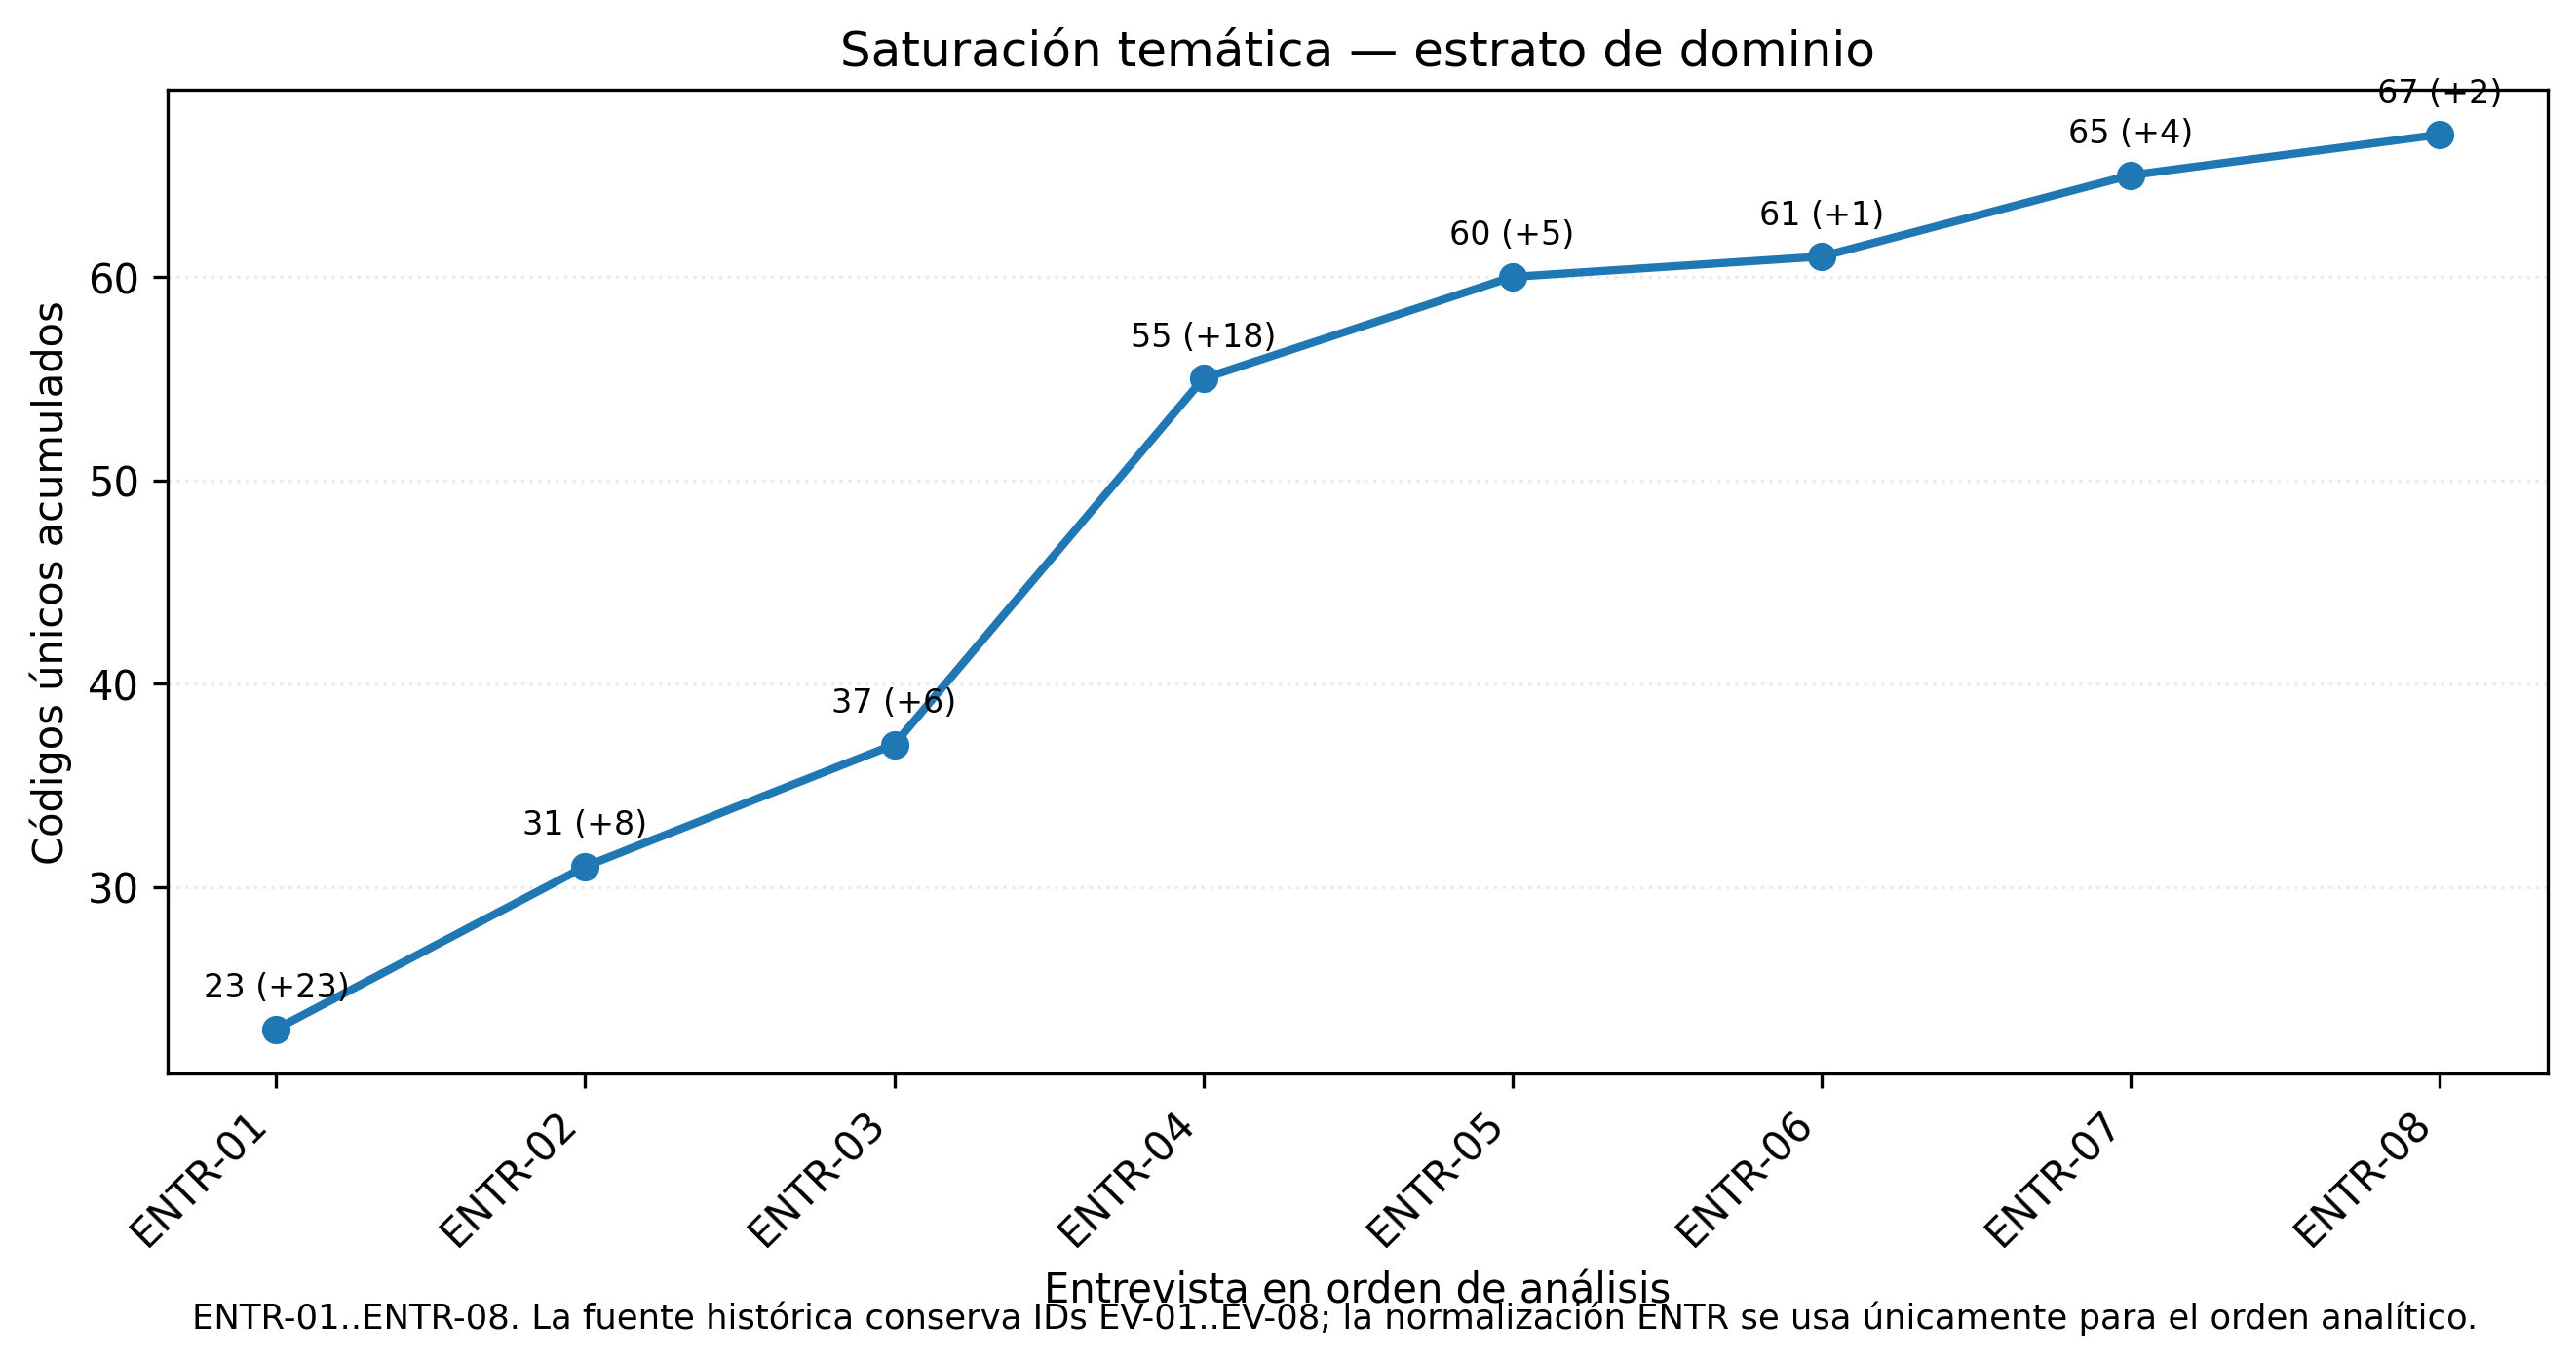
\includegraphics[width=0.85\linewidth]{../07_Datos/resultados/curva_saturacion_dominio.png}
\caption{Curva de saturaci\'on tem\'atica, estrato de dominio (\texttt{ENTR-01} a \texttt{ENTR-08}).}
\label{fig:saturacion-dominio}
\end{figure}

\begin{figure}[ht]
\centering
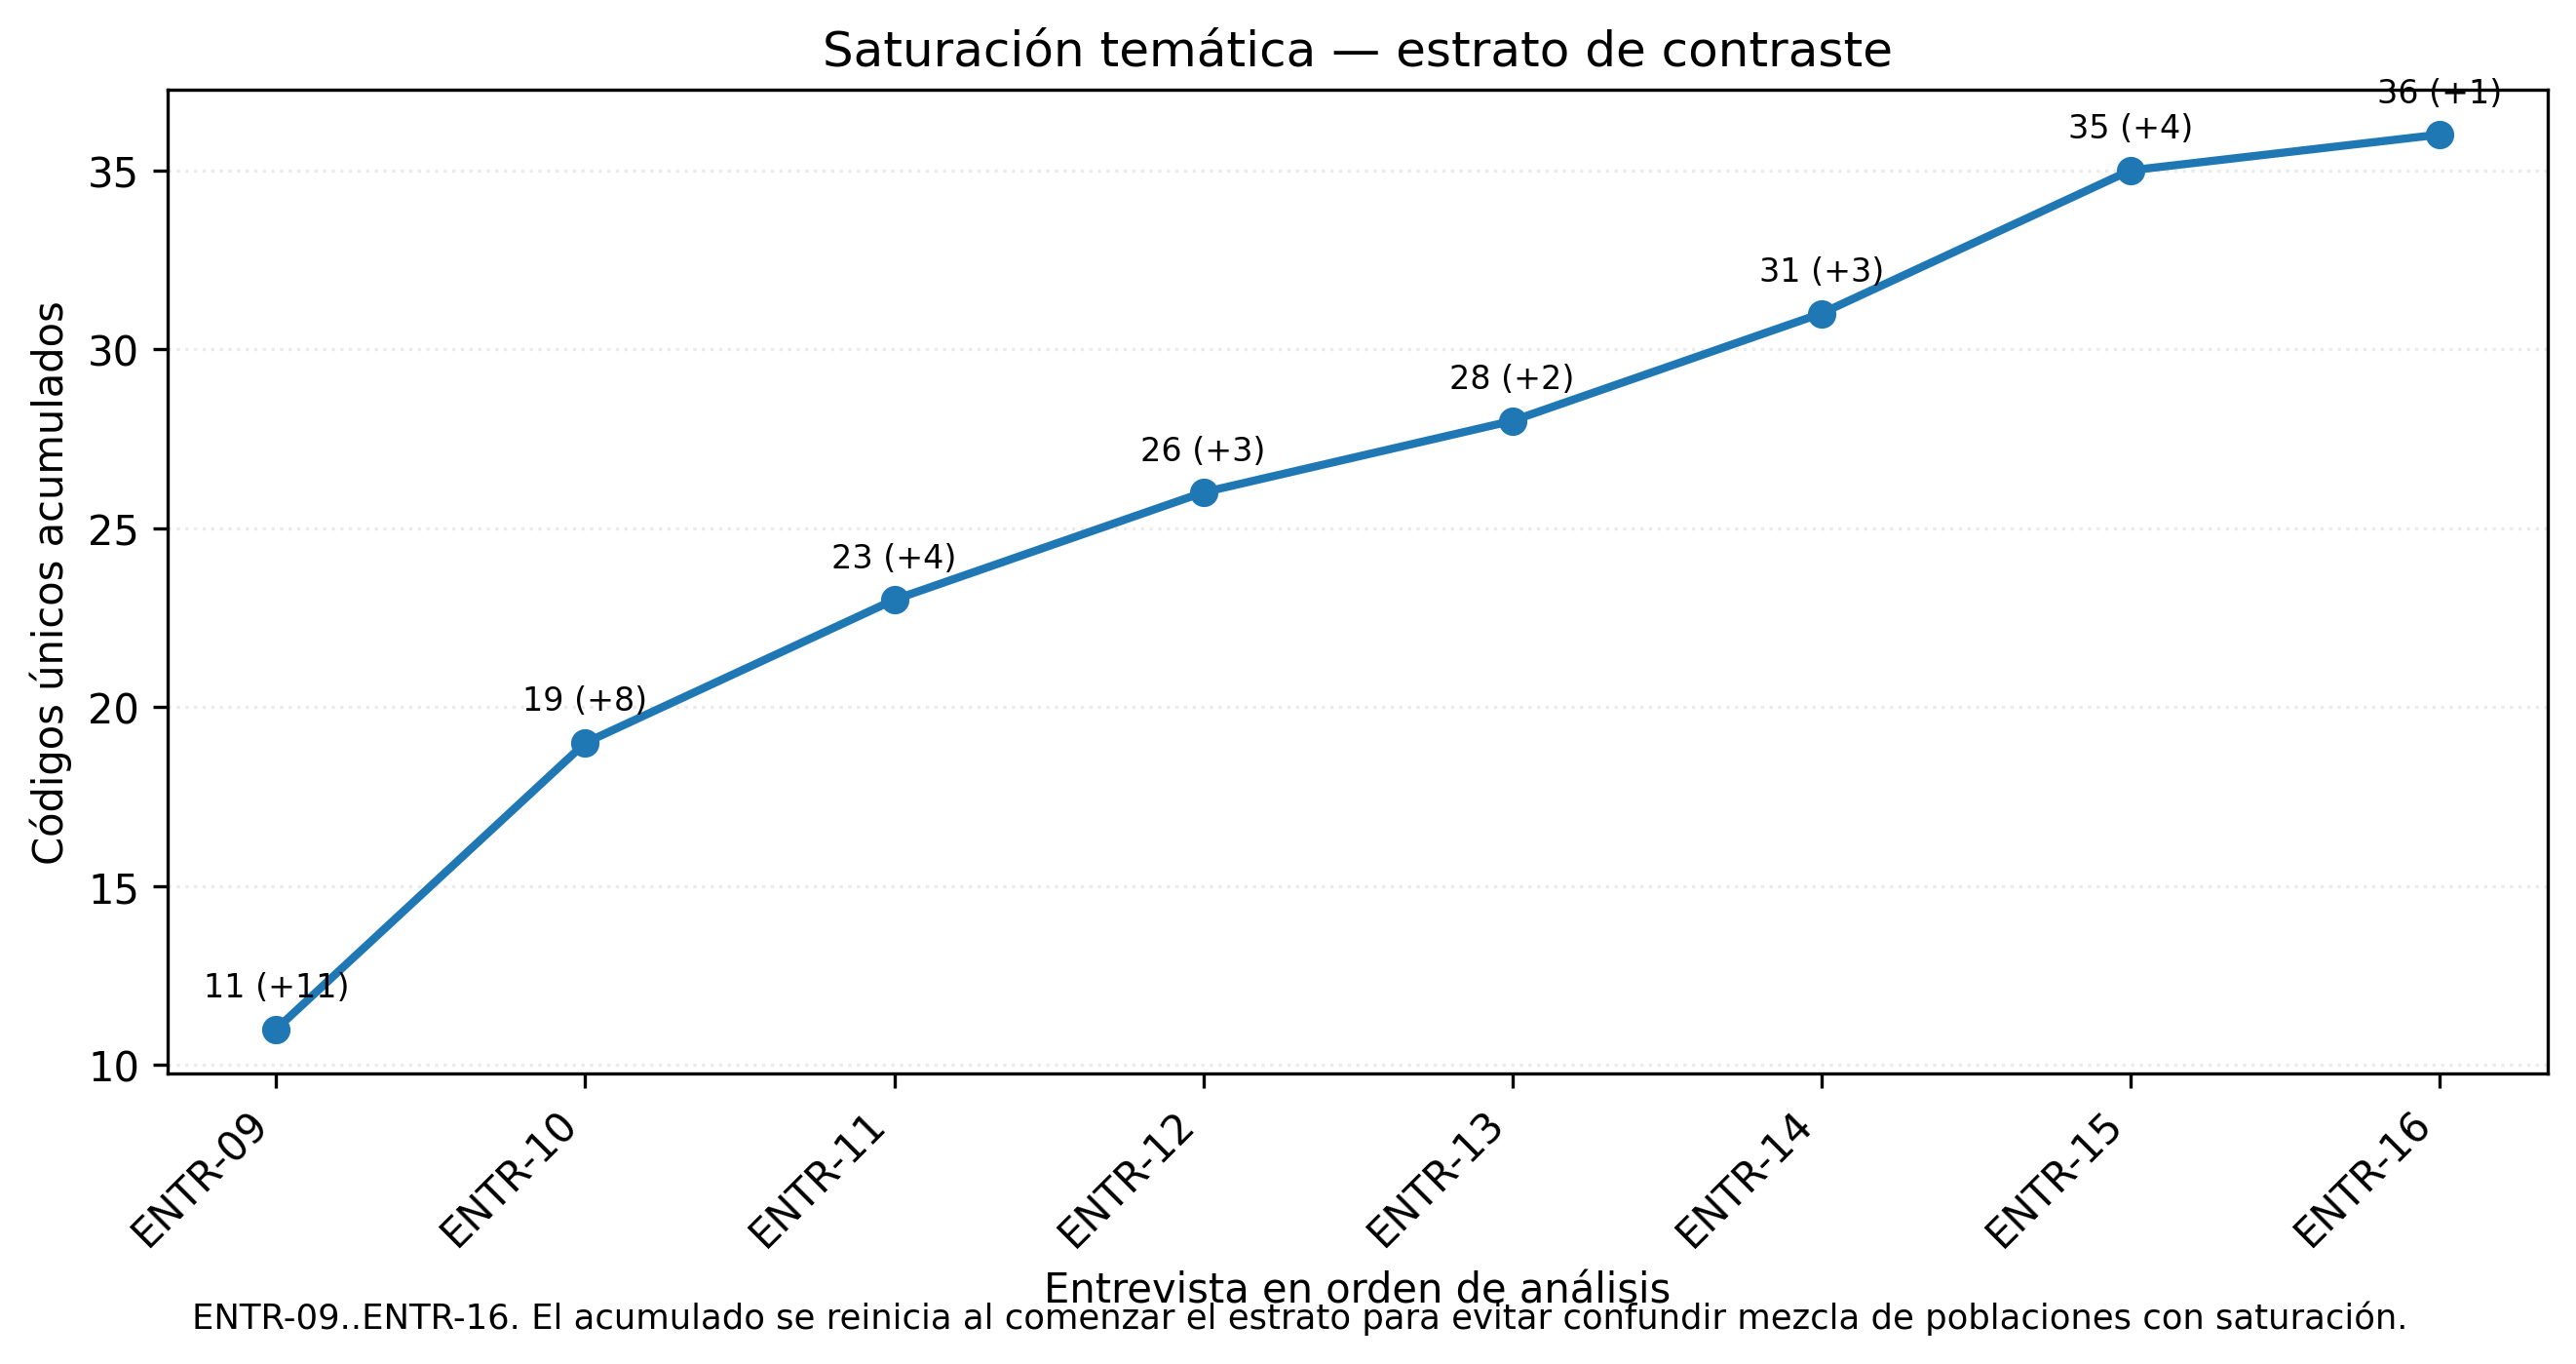
\includegraphics[width=0.85\linewidth]{../07_Datos/resultados/curva_saturacion_contraste.png}
\caption{Curva de saturaci\'on tem\'atica, estrato de contraste (\texttt{ENTR-09} a \texttt{ENTR-16}).}
\label{fig:saturacion-contraste}
\end{figure}

Esta vista agregada se conserva \'unicamente como descripci\'on del conjunto
completo de entrevistas y \textbf{no debe interpretarse como evidencia de
saturaci\'on homog\'enea entre las dos poblaciones}, dado que dominio y
contraste corresponden a perfiles con distinta relaci\'on con el objeto de
estudio. Las curvas de saturaci\'on por estrato se muestran en las
Figuras~\ref{fig:saturacion-dominio} y~\ref{fig:saturacion-contraste}; la
vista agregada, junto con la tabla completa de las 16 entrevistas, est\'a
disponible en \texttt{07\_Datos/resultados/}.

% =====================================================================
\section{Preguntas de investigaci\'on}
% =====================================================================

Marco PICOC: \textbf{poblaci\'on}, requisitos funcionales de un sistema
agroindustrial real; \textbf{intervenci\'on}, su generaci\'on mediante un modelo
grande de lenguaje desde una transcripci\'on anonimizada; \textbf{comparaci\'on},
los elicitados por el equipo humano desde el mismo material; \textbf{resultado}, la
puntuaci\'on en cinco dimensiones de calidad; \textbf{contexto}, un proyecto
acad\'emico de ingenier\'ia de requisitos en Ecuador.

\begin{description}
\item[RQ1.] ?`En qu\'e dimensiones de calidad difieren los requisitos funcionales
elicitados por un equipo humano de los generados por un modelo grande de lenguaje
a partir del mismo material fuente?
\item[RQ2.] ?`Cu\'al es el grado de acuerdo entre personas evaluadoras
independientes al valorar la calidad de requisitos funcionales sin conocer su
procedencia?
\end{description}

Para cada dimensi\'on $d$, la hip\'otesis nula sostiene que la distribuci\'on de
puntuaciones no difiere entre conjuntos. El contraste es \textbf{bilateral}: la
literatura reporta resultados mixtos y postular una direcci\'on sin base
constituir\'ia un sesgo de expectativa.

% =====================================================================
\section{Dise\~no del estudio}
\label{sec:diseno}
% =====================================================================

\subsection{Variables}

La \textbf{variable independiente} es el origen del requisito, nominal
dicot\'omica. Las \textbf{variables dependientes} son cinco puntuaciones ordinales
de 1 a 5, con descriptores por nivel y un ejemplo positivo y otro negativo en cada
uno: \emph{completitud} (presencia de los atributos de la plantilla),
\emph{ausencia de ambig\"uedad} (unicidad de interpretaci\'on),
\emph{verificabilidad} (existencia de un criterio objetivamente comprobable),
\emph{correcci\'on} (fidelidad al contenido de la transcripci\'on) y
\emph{consistencia interna} (ausencia de contradicci\'on con el resto del
conjunto). Se controlan el material fuente y la r\'ubrica, id\'enticos para ambos
conjuntos; la ceguera de las personas evaluadoras respecto del origen; y el orden
de presentaci\'on, aleatorizado con semilla registrada.

\subsection{Materiales y participantes}

Ambos conjuntos comprendieron veinticinco requisitos; el humano se extrajo del
cat\'alogo seleccionando los trazados a la evidencia de la entrevista fuente.
Participaron tres personas evaluadoras independientes, estudiantes de otro paralelo
de la misma asignatura sin participaci\'on en el proyecto. Las tres evaluaron los
50 requisitos en las cinco dimensiones previstas, generando 750 puntuaciones
ordinales. El n\'umero reducido de evaluadores constituye una limitaci\'on del
estudio.

\subsection{Procedimiento}

Verificada la anonimizaci\'on de la transcripci\'on fuente, el conjunto generado se
obtiene con una consigna literal \'unica, registrando modelo y versi\'on,
temperatura, \emph{top-p}, \emph{top-k}, semilla, fecha y hora, y la respuesta sin
edici\'on \cite{vogelsang2025}. Ambos conjuntos se transcriben a una plantilla
com\'un con identificadores neutros, sin marca de procedencia, y se mezclan en orden
aleatorio con semilla registrada; la correspondencia entre identificador y origen
se conserva aparte y no se entrega a las evaluadoras. Cada una punt\'ua todos los
requisitos de forma independiente. La procedencia se revela solo al completarse la
recolecci\'on.

% =====================================================================
\section{Plan de an\'alisis}
\label{sec:analisis}
% =====================================================================

\textbf{Ejecuci\'on del an\'alisis.} El an\'alisis se ejecut\'o despu\'es de
completar la recolecci\'on de las puntuaciones. Las decisiones metodol\'ogicas
principales utilizadas en esta etapa fueron fijadas antes de observar dichas
puntuaciones y quedaron documentadas en el repositorio. El protocolo p\'ublico
original no se modific\'o retroactivamente; las diferencias respecto de aquel
protocolo se conservan como desviaciones declaradas.

\subsection{Desviaci\'on respecto del plan original}

El protocolo original preve\'ia contrastes \textbf{apareados} sobre unos
veinticinco pares. Antes de recoger las puntuaciones se constat\'o que no exist\'ia
una correspondencia uno a uno metodol\'ogicamente justificable entre cada
requisito humano y uno generado por el modelo: ambos conjuntos proceden del mismo
material fuente, pero no describen necesariamente las mismas funciones. Por ello,
un contraste apareado habr\'ia impuesto una estructura inexistente.

La desviaci\'on qued\'o documentada en el repositorio antes de recoger las
puntuaciones experimentales y consisti\'o en:

\begin{enumerate}
\item tratar los dos conjuntos como \textbf{grupos independientes}, no apareados;
\item utilizar como an\'alisis principal un \textbf{modelo mixto de v\'inculo
acumulativo} para respuesta ordinal \cite{agresti2010}, con un modelo independiente
para cada una de las cinco dimensiones y la especificaci\'on
\[
\text{puntuaci\'on}_{1\text{--}5}
\sim
\text{origen}
+
(1 \mid \text{evaluador})
+
(1 \mid \text{requisito});
\]
\item utilizar origen como efecto fijo y evaluador y requisito como interceptos
aleatorios cruzados, con enlace log\'istico de probabilidades proporcionales;
\item reservar la prueba U de Mann--Whitney sobre la mediana por requisito,
acompa\~nada de $\delta$ de Cliff e intervalo de confianza al 95\,\%
\cite{cliff1993}, exclusivamente para el caso de que el modelo principal no
convergiera.
\end{enumerate}

Los cinco modelos principales convergieron sin advertencias, por lo que no fue
necesario ejecutar el an\'alisis de reserva. La implementaci\'on se realiz\'o con
el paquete \texttt{ordinal} de R, versi\'on 2026.7.26.

\subsection{Contrastes y acuerdo entre evaluadores}

Se aplic\'o la correcci\'on secuencial de Holm \cite{holm1979} sobre los cinco
contrastes del efecto de origen, uno por dimensi\'on, con $\alpha=0{,}05$. Se
reportan tanto los valores $p$ crudos como los corregidos.

Para RQ2 se utiliz\'o el $\alpha$ de Krippendorff con m\'etrica ordinal
\cite{hayes2007} como medida principal de acuerdo y el $\kappa$ de Cohen ponderado
cuadr\'aticamente \cite{cohen1968} por pares como medida secundaria.

\subsection{Potencia}

Como aproximaci\'on de sensibilidad, y no como potencia espec\'ifica del modelo
ordinal, se hab\'ia calculado previamente la potencia de un contraste convencional
de dos grupos independientes con $\alpha=0{,}05$ bilateral y $d=0{,}5$.
Veinticinco requisitos por grupo proporcionan una potencia aproximada de
\textbf{0,41}; alcanzar 0,80 requerir\'ia aproximadamente 64 requisitos por grupo.

Esta limitaci\'on se mantuvo durante la ejecuci\'on y la muestra no se ampli\'o
despu\'es de observar los resultados. Por ello, la interpretaci\'on considera
conjuntamente los estimadores, sus intervalos de confianza y los valores $p$, sin
equiparar ausencia de significaci\'on con equivalencia.

Todas las cifras que se presentan a continuaci\'on proceden de scripts
versionados en el repositorio.

% =====================================================================
\section{Resultados}
\label{sec:resultados}
% =====================================================================

El experimento incluy\'o 25 requisitos del conjunto humano y 25 requisitos
generados por el modelo. Tres evaluadores puntuaron los 50 requisitos en cinco
dimensiones, produciendo un total de 750 puntuaciones ordinales.

\subsection{RQ1: comparaci\'on entre requisitos humanos y generados por LLM}

Descriptivamente, las medias del conjunto humano fueron ligeramente superiores en
las cinco dimensiones. Para completitud y ausencia de ambig\"uedad la media fue
4,36 en humanos frente a 4,25 en LLM; para verificabilidad, 4,35 frente a 4,24;
para correcci\'on, 4,37 frente a 4,25; y para consistencia, 4,36 frente a 4,25.
La mediana fue 4 y el rango intercuart\'il 1 en ambos or\'igenes y en todas las
dimensiones.

La Tabla~\ref{tab:rq1} presenta el efecto de origen estimado por los modelos
ordinales mixtos. Humano se utiliz\'o como categor\'ia de referencia; por tanto,
un \emph{odds ratio} menor que 1 representa un desplazamiento estimado hacia
puntuaciones menores para LLM.

\begin{table}[ht]
\centering
\caption{Efecto de origen LLM frente a Humano en los modelos ordinales mixtos.}
\label{tab:rq1}
\small
\begin{tabular}{lrrrrr}
\hline
Dim. & $\beta$ & OR & IC 95\,\% OR & $p$ & $p_{\mathrm{Holm}}$ \\
\hline
COM & -0,267 & 0,766 & [0,416; 1,411] & 0,392 & 1,000 \\
AMB & -0,283 & 0,754 & [0,394; 1,442] & 0,393 & 1,000 \\
VER & -0,281 & 0,755 & [0,385; 1,481] & 0,414 & 1,000 \\
COR & -0,303 & 0,739 & [0,393; 1,390] & 0,348 & 1,000 \\
CON & -0,267 & 0,766 & [0,416; 1,411] & 0,392 & 1,000 \\
\hline
\end{tabular}
\end{table}

Los cinco coeficientes fueron negativos y los cinco \emph{odds ratios} inferiores
a 1. Sin embargo, todos los intervalos de confianza incluyeron 1 y ninguno de los
contrastes alcanz\'o significaci\'on estad\'istica. Tras la correcci\'on de Holm,
los cinco valores $p$ ajustados fueron 1,000.

Por tanto, en esta muestra \textbf{no se encontr\'o evidencia estad\'isticamente
significativa de diferencias de calidad entre los requisitos humanos y los
generados por el LLM en ninguna de las cinco dimensiones}. Este resultado no
demuestra equivalencia entre ambos or\'igenes.

Completitud y consistencia produjeron estimaciones id\'enticas porque las
puntuaciones observadas para ambas dimensiones fueron id\'enticas en el conjunto
analizado.

\subsection{RQ2: acuerdo entre evaluadores}

El acuerdo entre los tres evaluadores fue bajo en todas las dimensiones. La
Tabla~\ref{tab:rq2} muestra el $\alpha$ de Krippendorff con m\'etrica ordinal.

\begin{table}[ht]
\centering
\caption{Acuerdo interevaluador mediante $\alpha$ de Krippendorff ordinal.}
\label{tab:rq2}
\begin{tabular}{lrr}
\hline
Dimensi\'on & $\alpha$ de Krippendorff & IC 95\,\% \\
\hline
COM & -0,015 & [-0,192; 0,135] \\
AMB & -0,003 & [-0,181; 0,163] \\
VER & 0,027 & [-0,142; 0,168] \\
COR & -0,003 & [-0,174; 0,153] \\
CON & -0,015 & [-0,183; 0,135] \\
\hline
\end{tabular}
\end{table}

Los valores se situaron aproximadamente entre $-0,015$ y 0,027, es decir, muy
pr\'oximos a cero. Como medida secundaria, los valores de $\kappa$ ponderado
cuadr\'atico por pares oscilaron entre aproximadamente $-0,044$ y 0,297.

La Tabla~\ref{tab:kappa} muestra el promedio de $\kappa$ ponderado cuadr\'atico
por dimensi\'on, calculado sobre los tres pares de evaluadoras.

\begin{table}[ht]
\centering
\caption{Promedio de $\kappa$ ponderado cuadr\'atico por dimensi\'on (tres pares de evaluadoras, $n=50$ por par).}
\label{tab:kappa}
\begin{tabular}{lrr}
\hline
Dimensi\'on & $\kappa$ ponderado (promedio) & IC 95\,\% \\
\hline
COM & 0,073 & [-0,095; 0,213] \\
AMB & 0,095 & [-0,078; 0,241] \\
VER & 0,105 & [-0,056; 0,234] \\
COR & 0,083 & [-0,086; 0,223] \\
CON & 0,073 & [-0,086; 0,206] \\
\hline
\end{tabular}
\end{table}

En conjunto, RQ2 muestra que las personas evaluadoras presentaron un
\textbf{grado de acuerdo muy bajo} al aplicar la r\'ubrica a los requisitos
cegados.

% =====================================================================
\section{Discusi\'on}
\label{sec:discusion}
% =====================================================================

Los resultados de RQ1 muestran una direcci\'on consistente: las puntuaciones
estimadas favorecieron ligeramente al conjunto humano en las cinco dimensiones.
No obstante, la magnitud de la incertidumbre es suficiente para que todos los
intervalos de confianza de los \emph{odds ratios} incluyan 1. Con la muestra
disponible no es posible sostener que exista una diferencia estad\'isticamente
detectable entre los dos or\'igenes.

Este resultado debe distinguirse de una demostraci\'on de igualdad o equivalencia.
El estudio posee potencia limitada y fue dise\~nado como una comparaci\'on
exploratoria en un \'unico caso. La ausencia de significaci\'on puede ser
compatible tanto con diferencias peque\~nas como con una muestra insuficiente para
detectarlas con precisi\'on.

Desde una perspectiva aplicada, los requisitos producidos por el modelo obtuvieron
puntuaciones descriptivas cercanas a las del conjunto humano. Esto sugiere que un
modelo grande de lenguaje puede producir artefactos que, bajo determinadas
condiciones, reciban valoraciones de calidad similares. Sin embargo, los datos no
respaldan afirmar que el modelo pueda sustituir al proceso humano de elicitaci\'on:
el estudio eval\'ua un \'unico material fuente, un \'unico modelo y un \'unico
dominio.

El resultado de RQ2 es especialmente importante para interpretar RQ1. El acuerdo
interevaluador fue muy bajo en todas las dimensiones, lo que indica una variabilidad
considerable en la aplicaci\'on de la r\'ubrica. Aunque los modelos mixtos
incorporaron al evaluador como efecto aleatorio, esta falta de concordancia reduce
la precisi\'on con la que puede caracterizarse la calidad de cada requisito y debe
considerarse una amenaza a la validez de medici\'on y de conclusi\'on.

En consecuencia, la principal aportaci\'on emp\'irica del estudio no es demostrar
superioridad de uno de los dos or\'igenes, sino documentar que, bajo este dise\~no,
no se detectaron diferencias significativas y que la variabilidad entre
evaluadores constituye un componente relevante del problema de medici\'on.
Estudios posteriores deber\'ian ampliar el n\'umero de materiales fuente, modelos,
dominios y evaluadores, adem\'as de estudiar estrategias para aumentar la
consistencia en la aplicaci\'on de la r\'ubrica.

% =====================================================================
\section{Amenazas a la validez}
% =====================================================================

Se identificaron antes de la ejecuci\'on, seg\'un las categor\'ias de Wohlin et
al.\ \cite{wohlin2012}.

\textbf{Constructo.} La r\'ubrica puede no capturar la calidad de un requisito en su
totalidad; las dimensiones proceden de la literatura \cite{iso29148,montgomery2022} y
la limitaci\'on se declara. La escala ordinal comprime juicios heterog\'eneos, lo que
se mitiga con descriptores y ejemplos por nivel.

\textbf{Interna.} El conjunto humano lo elabor\'o el mismo equipo que ejecuta el
estudio; se mitiga con evaluaci\'on a ciegas, identificadores neutros y orden
aleatorizado con semilla registrada.

\textbf{Externa.} Un \'unico material fuente, dominio y modelo; no se generalizar\'a
m\'as all\'a del caso. Las evaluadoras son estudiantes y no profesionales: se declara
el perfil real y no se atribuir\'a a su juicio la condici\'on de experto.

\textbf{Conclusi\'on.} La potencia queda por debajo de 0,80, por lo que se reporta
el tama\~no del efecto con intervalo de confianza y no solo el valor $p$. Un acuerdo
bajo entre evaluadoras se reportar\'a igualmente y se discutir\'a como hallazgo. El cambio 
de dise\'on apareado a grupos independientes que agraba esta limitaci\'on de potencia se
declara como desviaci\'on prospectiva en \texttt{06\_Experimento/osf\_deviations.md}.

\medskip
\noindent\textbf{Amenazas del componente cualitativo que provee el material fuente.}
La transcripci\'on que act\'ua como material fuente y el cat\'alogo de requisitos del
que se extrae el conjunto humano proceden de un estudio de campo previo, cuya
interpretaci\'on se contrast\'o con las personas participantes mediante
\emph{member-checking}. Dos casos de ese proceso afectan a la confianza en dicho
material y se declaran aqu\'i; ambos constan en el registro de correcciones del
proyecto (\texttt{correcciones\_aplicadas.md}, casos D-02 y D-06).

\textbf{Instrumento.} Un enunciado de validaci\'on emple\'o el t\'ermino
\emph{herramienta}, que una de las tres personas consultadas interpret\'o como
herramienta f\'isica de trabajo y no como aplicaci\'on inform\'atica. El defecto es
de formulaci\'on y no de la persona participante, y redujo de tres a dos las
posiciones obtenibles sobre ese enunciado. Se reformul\'o el enunciado, se declara
la p\'erdida de una posici\'on y no se recab\'o de nuevo por encontrarse cerrado el
trabajo de campo.

\textbf{Credibilidad.} Un segundo enunciado recibi\'o posiciones incompatibles: dos
personas confirmaron una carencia de detalle en los reportes que una tercera neg\'o,
sin que exista evidencia documental independiente que permita adjudicar entre ambas
lecturas. La interpretaci\'on se conserv\'o por contar con el respaldo de dos de tres
fuentes y la divergencia se reporta sin conciliar, lo que limita la confianza en la
parte del material derivada de ese enunciado.

\textbf{Selecci\'on.} El analista l\'ider del equipo mantiene relaci\'on de
consanguinidad con dos de las personas participantes del estudio de campo:
\texttt{ENTR-02} en primer grado y \texttt{ENTR-07} en segundo grado, y condujo
personalmente ambas entrevistas. La circunstancia constituye una amenaza a la
validez por sesgo de selecci\'on y de deseabilidad social: el acceso a la
organizaci\'on se obtuvo por esa v\'ia y la muestra no es independiente del
equipo investigador, de modo que las posiciones recogidas en esas dos sesiones
pueden no ser equivalentes a las de un participante sin v\'inculo previo. La
declaraci\'on completa y las seis medidas de mitigaci\'on aplicadas constan en el
Ap\'endice A del ERS y en \texttt{09\_Etica/A06}; entre ellas, la prohibici\'on de
sustentar cualquier requisito exclusivamente en esas dos fuentes y la
triangulaci\'on obligatoria con las restantes entrevistas. No se retiran esas
dos entrevistas del corpus, pero ning\'un hallazgo descansa \'unicamente sobre
ellas y la limitaci\'on se reporta sin conciliar.

\textbf{Consentimiento retrospectivo del cuestionario.} El cuestionario aplicado
al personal operativo se distribuy\'o de forma an\'onima y no gener\'o, en su
momento, un registro de consentimiento informado individual verificable. Esta
limitaci\'on se regulariz\'o de forma posterior mediante un formulario de
consentimiento independiente y una sesi\'on complementaria con fotograf\'ias
reales, aplicados a un subconjunto de participantes localizables y no a la
totalidad de quienes respondieron el cuestionario original. El consentimiento
complementario no se vincula con ninguna respuesta espec\'ifica de las 62
respuestas an\'onimas, por lo que no puede utilizarse para validar
retrospectivamente el conjunto completo; esta limitaci\'on se declara y no se
subsana en su totalidad, y se detalla en
\texttt{02\_Evidencias/Cuestionario/Respuestas/readme.md} y
\texttt{02\_Evidencias/Cuestionario/Consentimiento\_Complementario/readme.md}.
% =====================================================================
\section{Estado y contribuci\'on}
\label{sec:estado}
% =====================================================================

El protocolo experimental fue registrado p\'ublicamente antes de la ejecuci\'on
del experimento humano--LLM y antes de recoger sus puntuaciones. El material
fuente de entrevistas, en cambio, ya exist\'ia en ese momento; por ello, el
registro no se presenta como prerregistro del trabajo de campo previo ni del
proyecto completo.

El experimento comparativo se encuentra \textbf{ejecutado y analizado}. Se
evaluaron 25 requisitos humanos y 25 requisitos generados por el modelo mediante
tres evaluadores independientes y una r\'ubrica de cinco dimensiones. Los
resultados se reportan con independencia de que los contrastes hayan resultado
significativos.

La contribuci\'on es doble: por una parte, aporta evidencia emp\'irica sobre la
calidad percibida de requisitos funcionales humanos y generados por un modelo
grande de lenguaje en un dominio agroindustrial; por otra, documenta un
procedimiento reproducible de cegado, evaluaci\'on ordinal y an\'alisis del acuerdo
entre evaluadores.

El registro p\'ublico no equivale a un \emph{Registered Report} con aceptaci\'on
en fase~1, puesto que el dise\~no no fue sometido a revisi\'on editorial previa.
Las desviaciones respecto del plan original se documentan expl\'icitamente y el
protocolo registrado no se modifica retroactivamente.
% =====================================================================
\section*{Declaraci\'on de disponibilidad de datos}
% =====================================================================

El registro del protocolo est\'a disponible en Open Science Framework
(\url{https://osf.io/4z35d/}). El repositorio p\'ublico del proyecto se encuentra
en \url{https://github.com/gleiston-guerrero/SIMPA_ISR401}.

Como material complementario del proyecto se mantiene un dep\'osito con
estad\'istica descriptiva agregada del cuestionario aplicado al personal operativo
(\href{https://doi.org/10.5281/zenodo.22236500}{10.5281/zenodo.22236500}).
Dicho dep\'osito corresponde a un componente previo del proyecto y no constituye
el dep\'osito de los datos experimentales humano--LLM.

El repositorio del proyecto contiene los artefactos versionados utilizados para
el experimento, incluidos los conjuntos cegados y procesados, los scripts de
preparaci\'on y an\'alisis y los resultados estad\'isticos reportados en este
manuscrito. La correspondencia confidencial utilizada durante el cegado se
mantuvo separada del repositorio p\'ublico durante la evaluaci\'on.

Las personas evaluadoras se identifican mediante c\'odigos y no por sus nombres
en los datos anal\'iticos. La gesti\'on y publicaci\'on de sus datos debe mantenerse
de acuerdo con el consentimiento aplicable y con las medidas de privacidad
documentadas en el proyecto. La organizaci\'on de los artefactos sigue los
principios FAIR \cite{wilkinson2016}.

El cuestionario aplicado al personal operativo se distribuy\'o de forma
an\'onima mediante Google Forms: el equipo envi\'o el enlace al administrador
de la unidad productiva, quien lo comparti\'o con los trabajadores. Se
recibieron 62 respuestas. El car\'acter an\'onimo del instrumento no gener\'o,
en su momento, un registro de consentimiento informado individual y
verificable independiente de las respuestas. Esta limitaci\'on se
regulariz\'o de forma posterior y complementaria mediante un formulario de
consentimiento informado independiente, aplicado en septiembre de 2026 a un
grupo de participantes localizables, junto con fotograf\'ias originales de
dicha sesi\'on complementaria. Dicho consentimiento posterior y las
fotograf\'ias correspondientes no sustituyen ni se presentan como parte de
la aplicaci\'on original del cuestionario, y no existe ning\'un mecanismo que
vincule una respuesta an\'onima espec\'ifica con la identidad de un
participante del consentimiento complementario.

% =====================================================================
\section*{Uso de tecnolog\'ias asistidas por inteligencia artificial}
% =====================================================================

\textbf{Como objeto de estudio.} Uno de los conjuntos experimentales fue generado
mediante un modelo grande de lenguaje a partir del material fuente definido para
el experimento. La consigna, los par\'ametros disponibles de ejecuci\'on y los
artefactos resultantes se documentaron dentro del flujo experimental.

\textbf{Como apoyo al trabajo acad\'emico.} Durante la preparaci\'on y revisi\'on
del manuscrito se utilizaron asistentes de inteligencia artificial, incluidos
Claude (Anthropic) y ChatGPT (OpenAI), como apoyo para redacci\'on,
reestructuraci\'on, revisi\'on de coherencia y formulaci\'on de interpretaciones.

Los asistentes no sustituyeron la ejecuci\'on del an\'alisis estad\'istico. Las
cifras, estimadores, intervalos de confianza, valores $p$ y medidas de acuerdo
reportados proceden de los datos reales y de los scripts versionados del proyecto.
Las personas autoras revisaron las interpretaciones propuestas y mantienen la
responsabilidad sobre las decisiones metodol\'ogicas, la verificaci\'on de los
resultados y las afirmaciones finales del manuscrito.

Las referencias bibliogr\'aficas deben ser contrastadas con sus fuentes
bibliogr\'aficas o editoriales originales y con sus identificadores persistentes
cuando est\'en disponibles antes de una eventual presentaci\'on externa.

% =====================================================================
\section*{Agradecimientos y conflicto de intereses}
% =====================================================================

Las personas autoras agradecen a la unidad productiva participante y a su personal
el tiempo dedicado a las entrevistas y el acceso a la documentaci\'on operativa. Agradecemos
asimismo al docente supervisor del proyecto por la orientaci\'on acad\'emica y metodol\'ogica durante
el desarrollo del estudio. Una de las personas autoras mantiene una relaci\'on de parentesco con el representante de la organizaci\'on participante; la circunstancia se declar\'o ante la instancia
acad\'emica antes del trabajo de campo y se adoptaron medidas de mitigaci\'on
documentadas. No se declaran otros conflictos de intereses.

\enlargethispage{3\baselineskip}
\bibliographystyle{splncs04}
\bibliography{referencias}

\end{document}
